%--------------------------------------------------
%	DOCUMENT CONFIGURATION
%--------------------------------------------------

\documentclass[a4paper, 10pt]{article}
\usepackage[utf8]{inputenc}
\usepackage[T1]{fontenc}
\usepackage[french]{babel}
\usepackage[margin=1in]{geometry}
\usepackage{import}
\usepackage{hyperref}
\usepackage{amsmath, amssymb, mathtools}
\usepackage{graphicx}
\usepackage[subpreambles=true]{standalone}
\usepackage{cleveref}
\usepackage[table]{xcolor}
\usepackage{titlesec}
\usepackage{listings}
\usepackage{subcaption}
%-----------------------------------------------
% DOCUMENT CONFIG
%-----------------------------------------------
%images storage 
\graphicspath{ {./images/} }
% Add point after title number
\titleformat{\section}[block]{\sc\bfseries\center\Large}{\thesection.}{0.5em}{}
\titleformat{\subsection}[block]{\sc\bfseries\center}{\thesubsection.}{0.5em}{}
\titleformat{\subsubsection}[block]{\sc\bfseries\center}{\thesubsubsection.}{0.5em}{}
\lstset{
frame=single,
basicstyle=\ttfamily\small,
numbers=left,
%numbersep=5pt,
literate=%
{é}{{\'e}}1
{à}{{\`a}}1
}

\begin{document}
	\paragraph{}L'application Android  été développé Sous l'IDE Android Studio 3, avec l'API Android 26, mais supportant les versions Plus vielles jusqu'à la version 16 de l'api, ce qui nous permet de l'installer sur 99\% des appareils Android sur en circulation. Le code de l'application a été entièrement managé avec Git, il est d'ailleurs  disponible a l'adresse suivante :  \url{https://github.com/tndnc/pandroid/tree/master/equity}. 
	\paragraph{}Le but de l'application est le suivant : l'utilisateur doit pouvoir sélectionner un niveau, jouer une partie et noter le niveau en question. quand a nous, il faut qu'il soit possible mettre a jour la liste des niveaux facilement lors des mises a jour de l'application, et que les notes et donnés provenant du déroulement d'une parte soit récupérables via internet sur un document Google sheets(via Google Sheets API v4).  
	
	\subsection{Composant Android}
	\paragraph{} Une application android s'organise en plusieurs composants , nous allons en présenter certains dans la section suivante pour pouvoir présenter l'application et ses fonctionnalités avec plus d'aisance, nous allons notamment nous concentre sur le concept d'activité qui est nécessaire pour pouvoir présenter l'interface.
\hfill \break
\begin{itemize}
	\item Une Activité Android correspond a une fenêtre d'une application, chaque application est composé d'au moins une activité et la navigation a l'intérieur de l'application se fait en changeant d'activité. Une Activité dispose d'une interface utilisateur graphique  par un layout faite de vues (ex : un bouton) et elle répond à des évènements (ex : lancer une nouvelle activité).
	\item Un layout est un ficher XML qui est chargé par une activité lorsque celle-ci est crée, il contiens des vues qui permettent de définir les éléments graphiques (vues) de l'activité comme par exemple des boutons.
\end{itemize}
	\subsection{Structure de l'application}
Notre application est donc composé de six activités que nous allons présenter dans ce paragraphe :
\hfill \break
\begin{itemize}
 \item \texttt{MainMenuActivity} : l'activité principale de l'application, lorsque celle ci est ouverte l'utilisateur arrive sur l'écran qui correspond au Menu Principal, il a ensuite la possibilité d'ouvrir de sélectionner un des quartes boutons du layout pour effectuer les actions suivantes : Ouvrir le menu de sélection des niveaux ,lancer le tutoriel , modifier sons profile et Ouvrir L'onglet About.
 \item \texttt{LevelSelectActivity} : l'activité de sélection des niveaux,la liste des niveaux est affiché, catégorisé par le nombre d'agents de chacun des niveaux l'utilisateur a la possibilité lancer chacun des niveaux présentés.
 \item \texttt{UserProfileActivity} : Cette activité remplace la \texttt{MainMenuActivity} lors du premier lancement de l'application, elle comporte deux zones d'entré de texte qui permettent a l'utilisateur de rentrer sa formation et son age, ses données serons ensuite utilisé lors de l'apprentissage de la difficulté des niveaux, on note que l'utilisateur a la possibilité lancer cette activité depuis le menu principal ou de ne pas remplir les champs de texte si il ne désire pas partager ces informations. 
 \item\texttt{AboutActivity} : un bref résumé de l'objectif de notre projet, de la raison pour laquelle a été développé l'application.
 \item\texttt{TutorialActivity} : le tutoriel du jeu, on y trouve une description de l'interface de jeu, la définition de ce qu'est un agent jaloux, les modalités de victoire d'une partie ainsi que des captures d'écran pour illustrer nos propos.
 \item \texttt{GameActivity} : l'activité ou se déroule la partie, elle est composé principalement d'un canevas sur lequel est afficher l'interface de jeu, et deux autres vues qui permettent d'afficher le nom du niveau et un bouton permettant d'afficher les acteurs jaloux.
 \end{itemize}  
 
\begin{figure}[h!]
    \centering
    \begin{subfigure}[a]{0.23\textwidth}
        \centering
        
\includegraphics[height=2.5in]{abou}
        \caption{sélection}
    \end{subfigure}
        \begin{subfigure}[b]{0.23\textwidth}
        \centering
        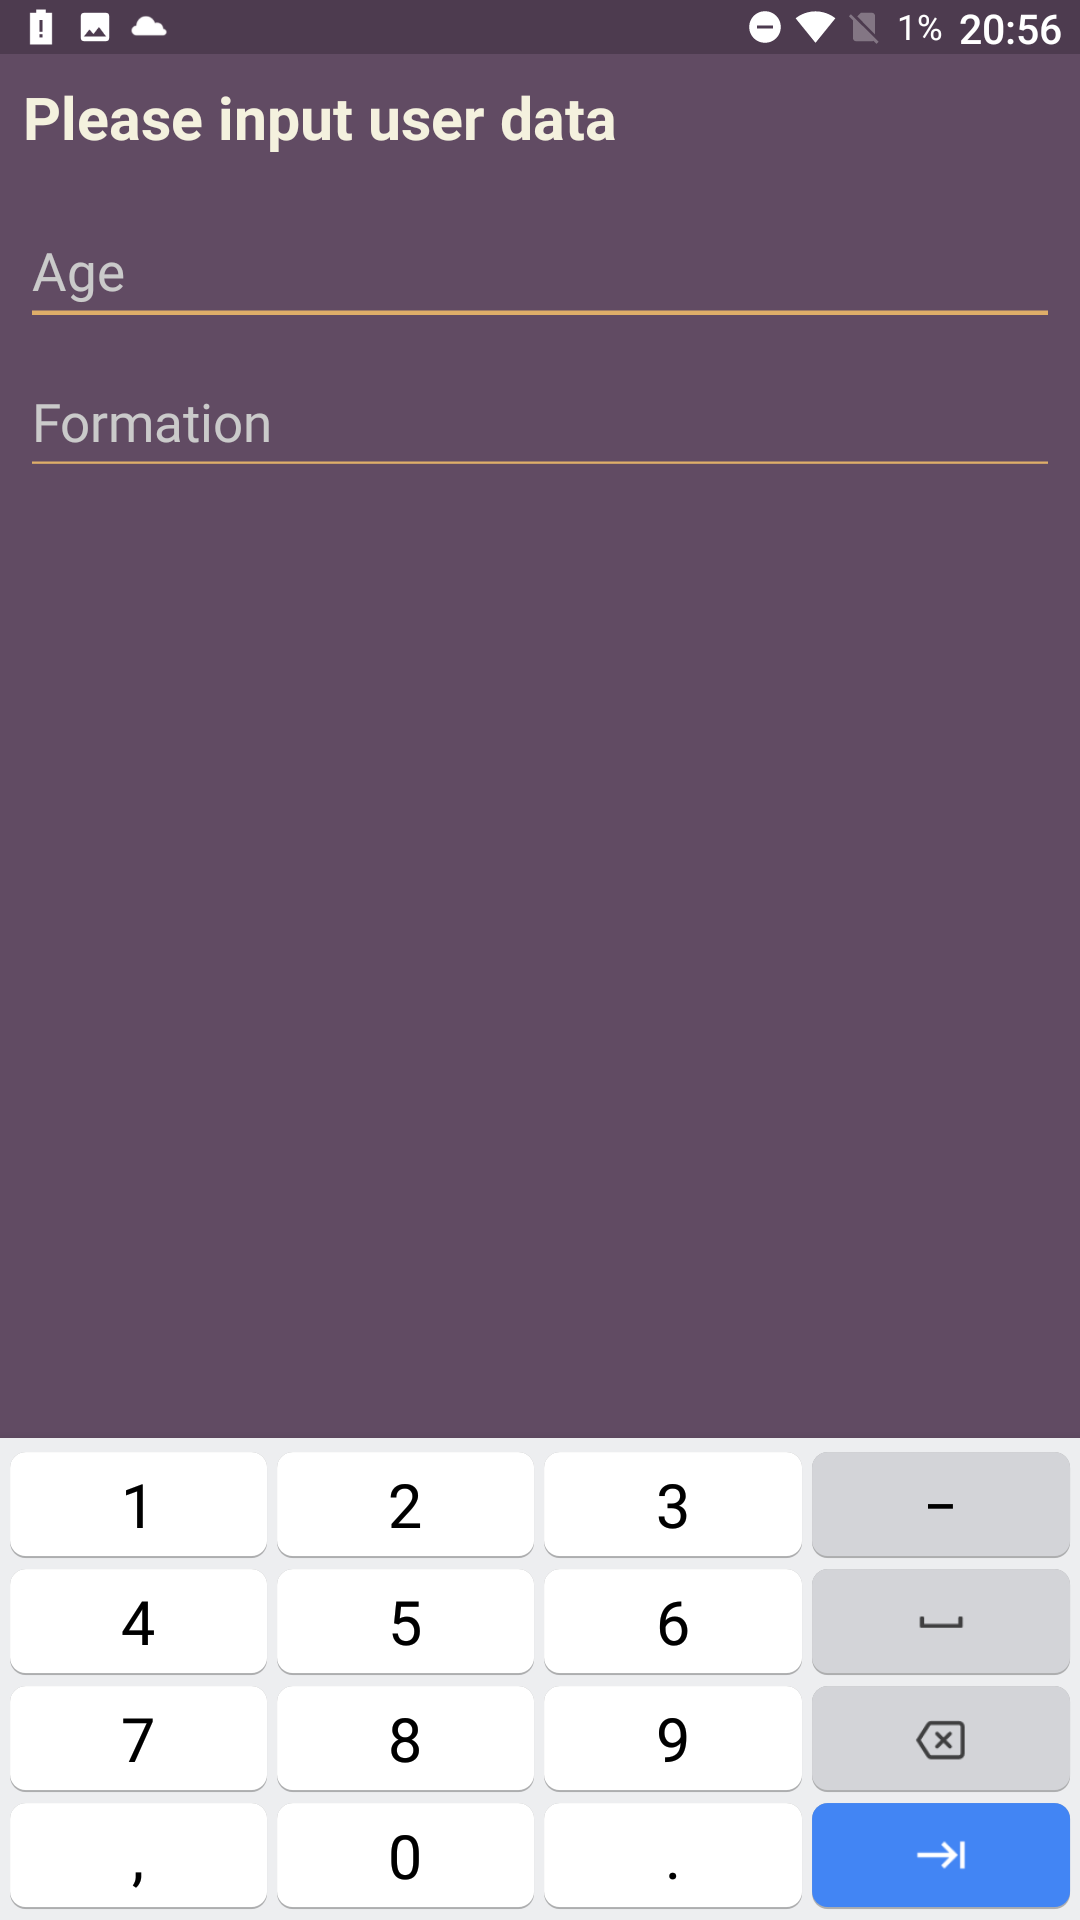
\includegraphics[height=2.5in]{infor}
        \caption{sélection}
    \end{subfigure}%
        \begin{subfigure}[c]{0.23\textwidth}
        \centering
        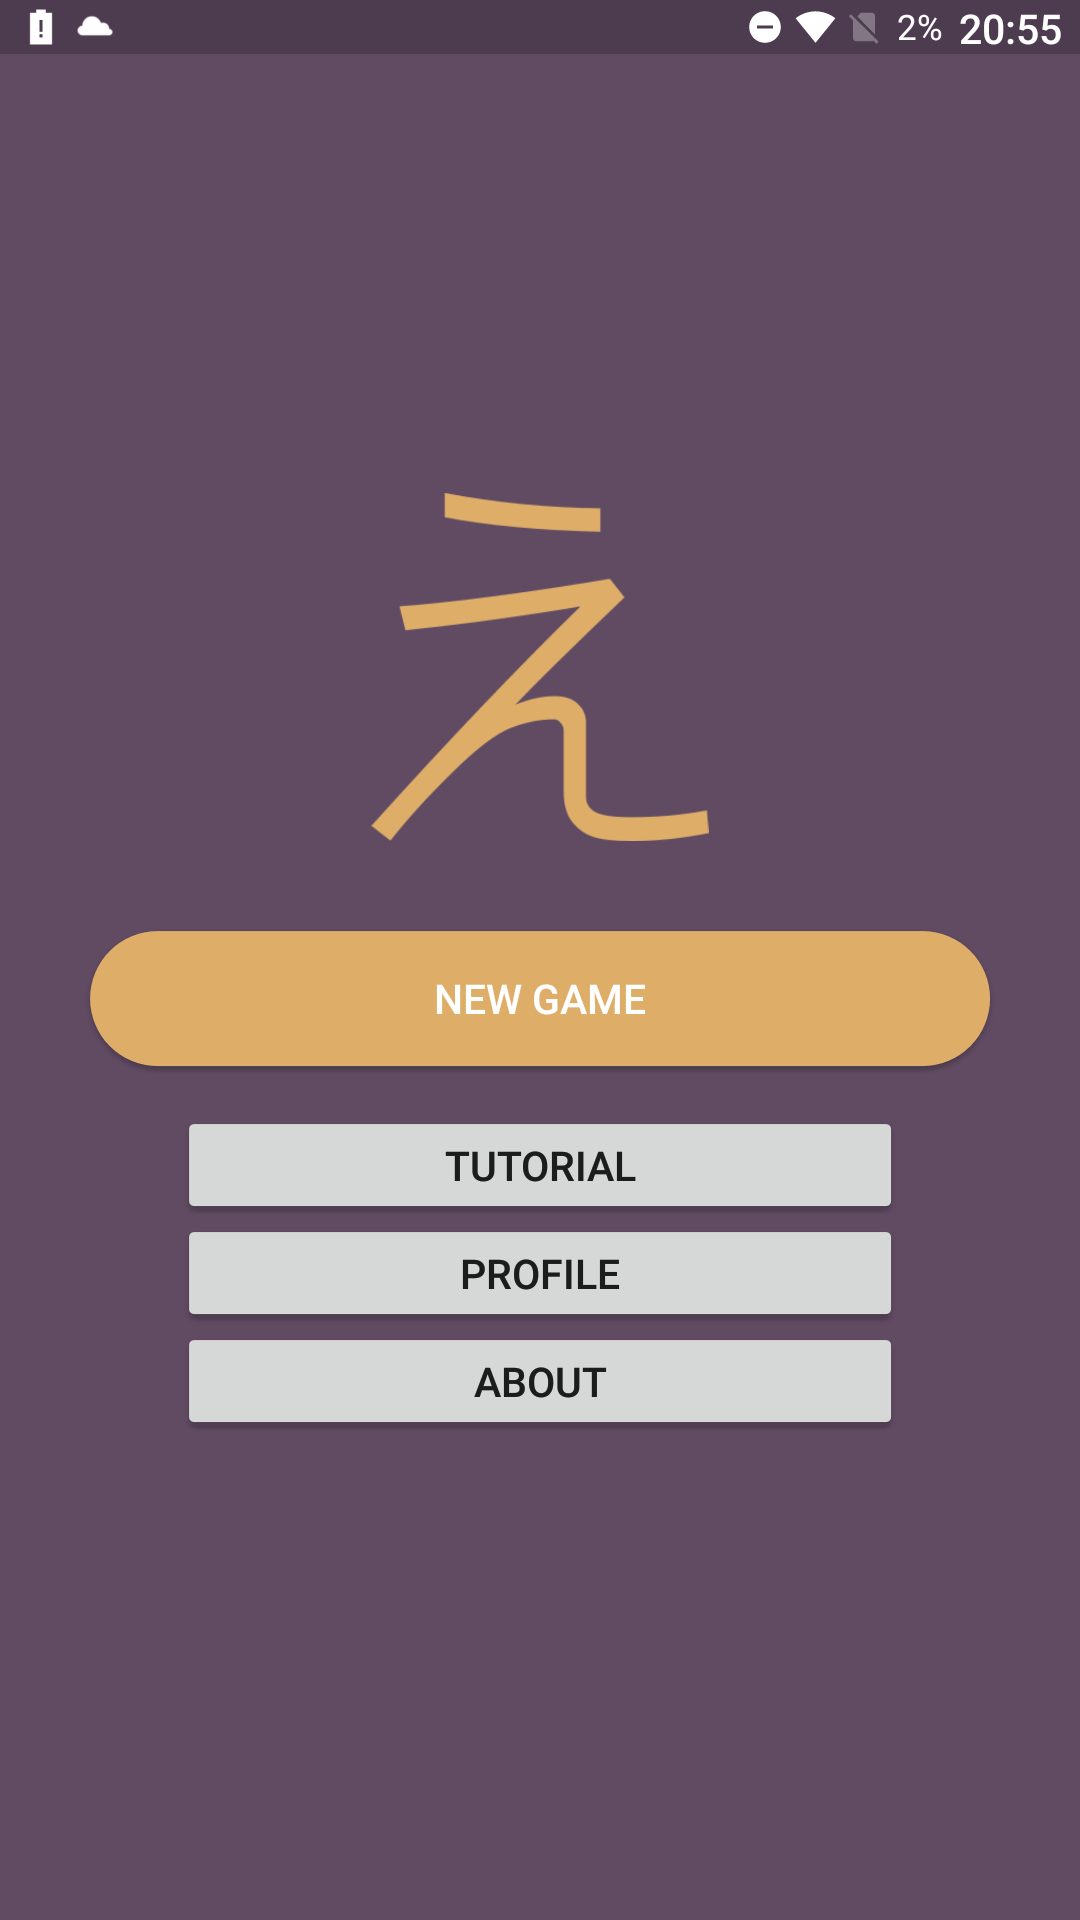
\includegraphics[height=2.5in]{main}
        \caption{affichag}
    \end{subfigure}%
    \begin{subfigure}[d]{0.23\textwidth}
        \centering
        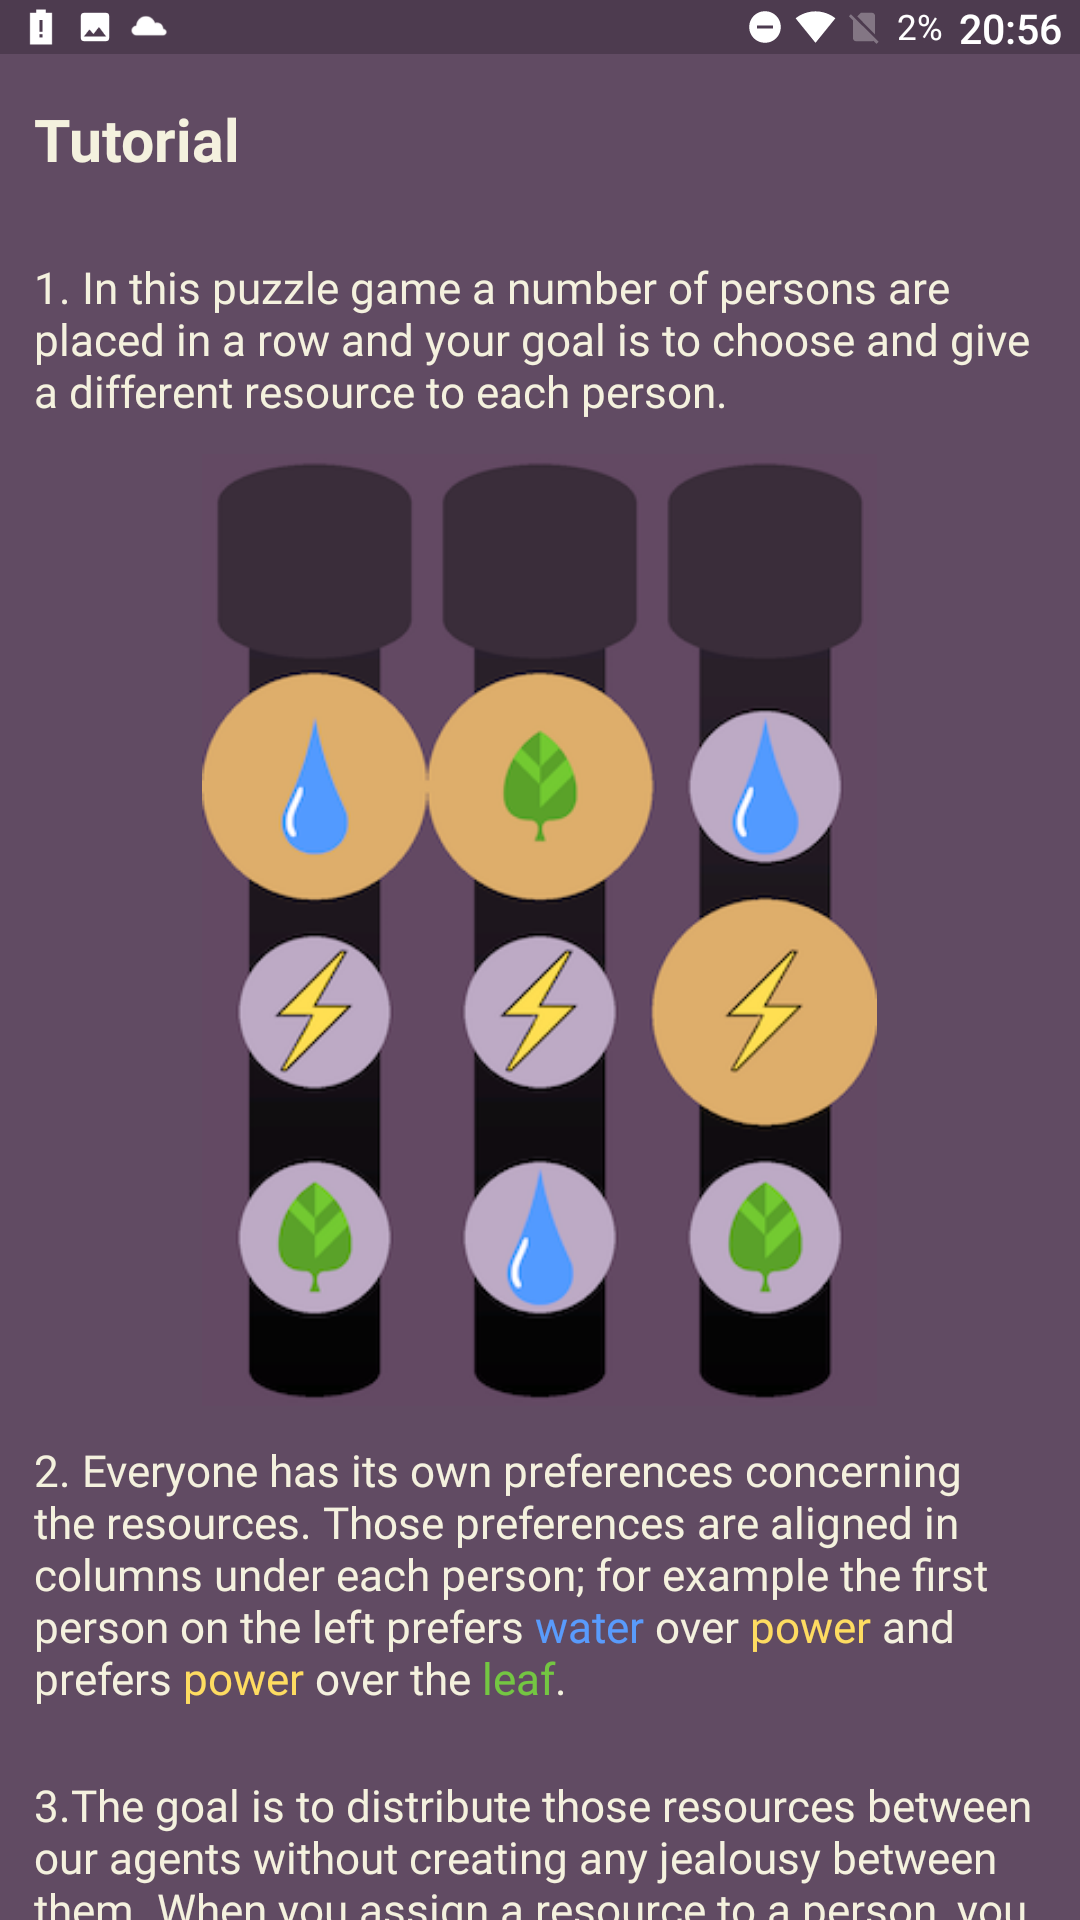
\includegraphics[height=2.5in]{tuto}
        \caption{victoire}
    \end{subfigure}
    \caption{Exemple Gameview}
\end{figure}
 
	\subsection{Le modèle du jeu}

\paragraph{}
la représentation théorique du jeu est stocké dans l'application Android sous le package \texttt{models}, On trouve dans ce package la classe \texttt{Model} qui est appelé des lors qu'il est nécessaire de faire une modification du modèle, par exemple l'assignation d'une préférence a un des agents ou encore lorsqu'il faut récupéré des informations par rapport au jeu, comme le nombre d'agents d'un niveau. La classe 
\texttt{Model} store en effet la grille qui représente le niveau en question, comprenant les agents et les préférences. Le package model contiens aussi la définition de l’interface IPiece de laquelle découle les Classe Preference et Actor qui représente respectivement les préférences et les agents.
 \begin{itemize}
\item définition d'une Pièce (Interface \texttt{IPiece}) : L’interface IPiece est composé de deux méthodes, la méthode getId qui retourne l'identifiant de la pièce et la méthode get position qui permet de retourner la position de la pièce sous forme d’un objet position qui contient les l’indices de la ligne et de la colonne dans lesquelles se trouve la pièce.   
\item définition d’un Acteur (Class \texttt{Actor}) :La classe Actor implémente l'interface IPiece et toute ses méthodes, elle représente les agents du jeu.                                                                                                                                                                                                                                                                                                                                      
\item définition d’une Préférence ( Class \texttt{Préférence}) : La classe Préférence implémente également l’interface IPiece, on y ajoute cependant la deux entier, value : qui permet de déterminer de quel type est cette préférence et selecteby : qui permet de savoir si cette préférence est sélectionnée par un des agents et par quel agent elle l’est. 
\end{itemize}
\hfill \break
\begin{lstlisting}
    private boolean isJealous(Preference[] P1,Preference[] P2){
        if (P1[0] == null){
            return false;
        }
        Preference P2pref = null;
        Preference P1pref = null;
        for (Preference pref:P1){
            if(pref.getSelectedby() != -1){
                P1pref = pref;
            }
        }
        for(Preference pref:P2){
            if(pref.getSelectedby() != -1){
                P2pref = pref;
            }
        }
        if(P1pref == null || P2pref == null){
            return false;
        }
        for(Preference pref:P2){
            if(pref.getValue() == P1pref.getValue()){
                if(pref.getPos().getCol() < P2pref.getPos().getCol()){
                    return true;
                }
            }
        }
        return false;
    }
\end{lstlisting}
Fonction de détection de la jalousie 

	\subsection{Design interface}
	
\paragraph{}
L’interface centrale de  l’application, l’ère de jeu de equity est un des composants principaux du projet et a suivis un certain nombre d'itérations qui seront décrites dans la partie suivante le premier objectif de cette interface était de pouvoir représenter le jeu sur un écran de smartphone en mode portrait
\paragraph{}
Il a été déterminé très tôt dans le projet qu’une visualisation sous forme de grille serait nécessaire chaque case de la grille représentant une préférence d’un des agents. Il a ensuite été décidé que les agents, représentés par des carrés, serait placé sur la gauche de la grille et leur préférences, représenté par des cercles, sur la même ligne que l’agent avec son objet préféré sur la gauche le plus proche de lui.
\paragraph{}
Il a ensuite été décidé que pour afficher la sélection d’une préférences par un des agents, Un cercle de la couleur de l’agent serait dessiné derrière le cercle représentant la préférence en question, l'utilisateur peut donc choisir de sélectionner une certaine préférence en touchant l'icône correspondante. On note que le processus de sélection des ressources empêche de sélectionner plusieurs ressources pour un seul agent. A ce stade l’application est fonctionnelle.
\paragraph{}
La dernière Modification Structurelle de l’IHM consiste a eu Pour but d’optimiser l’espace qui est alloué  à l’affichage des Préférences des agents : L'affichage de la grille de jeu été pivoté pour que les agents se trouvent en haut de l'écran, l'alignement des préférences se faisant donc de haut en bas, ce changement a donc permis d'utiliser une plus grande partie de la hauteur de l'écran du smartphone, en effets cette rotation de la grille a permis d'économiser une colonne en ajoutant une ligne ce qui est plus adapté à l’affichage en mode portrait.
\paragraph{}
les modifications suivantes de l’activité ont été des modification soit esthétiques soit relevant de l’ajout de features, tout d’abord l’interface a suivis un redesign complet, une harmonisation des couleurs et des formes pour la représentation de la plupart des éléments à dessiner. L’ajout de barres verticales pour chacun des agents, ce qui facilite la lisibilité et  L’ajout de l’identifiant du niveau.
\paragraph{}
    Après avoir testé cette interface Nous avons décidé que pour améliorer l'expérience de jeu nous devions rendre la détection d’affectation erroné plus aisée. Nous avons donc implémenté les solutions Suivantes :
 l’affichage d’une couleur différente sur les ressources sélectionnés par deux agents ce qui permet au joueur de remarquer immédiatement si une assignation des ressources est impossible
La possibilité d’afficher en rouge les colonnes des agents jaloux, Notons que cette fonctionnalité facilite grandement le jeu, elle est donc désactivé par défaut et le joueur a la possibilité d’appuyer sur un bouton pour activer cet affichage.
\paragraph{}
    Ces deux fonctionnalités facilitent grandement le gameplay mais nous pensons que ce compromis permet une expérience de jeu plus fluide et agréable pour l’utilisateur, un point qui nous semble essentiel pour la distribution de l’application. 


	\subsection{Interface GameView}
	
L'interface centrale de  l'application, l'ère de jeu de equity est un des composants principaux du projet, le canevas utilisé pour dessiner les agents et leur préférence s'organise de la façon suivante : les agents sont placé en haut de la surface sur une ligne horizontale, et leurs préférences sont arrangés verticalement, leur objet préféré étant le premier en partant du haut, derrière chaque agent est dessiné une bande verticale sur laquelle sont aligné les préférences 
\begin{figure}[h!]
    \centering
    \begin{subfigure}[a]{0.23\textwidth}
        \centering
        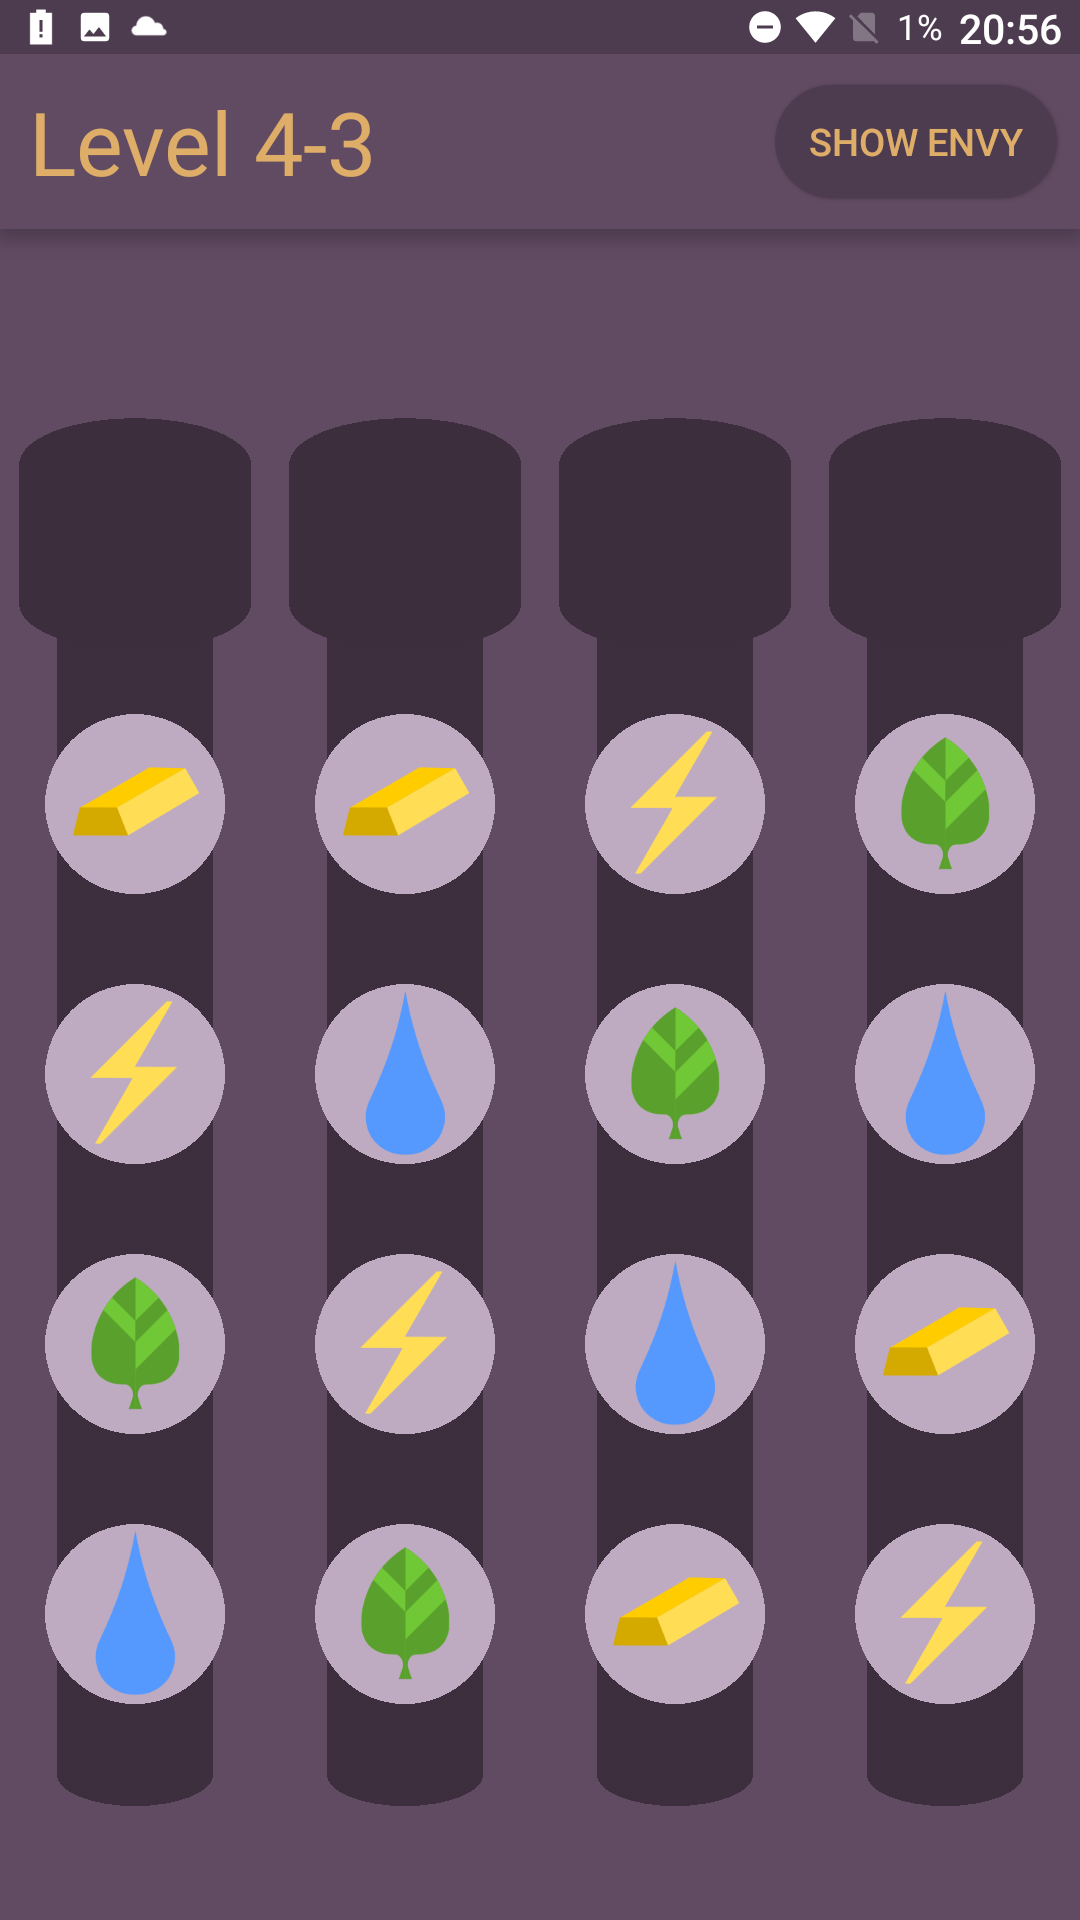
\includegraphics[height=2.5in]{g1}
        \caption{sélection}
    \end{subfigure}
        \begin{subfigure}[b]{0.23\textwidth}
        \centering
        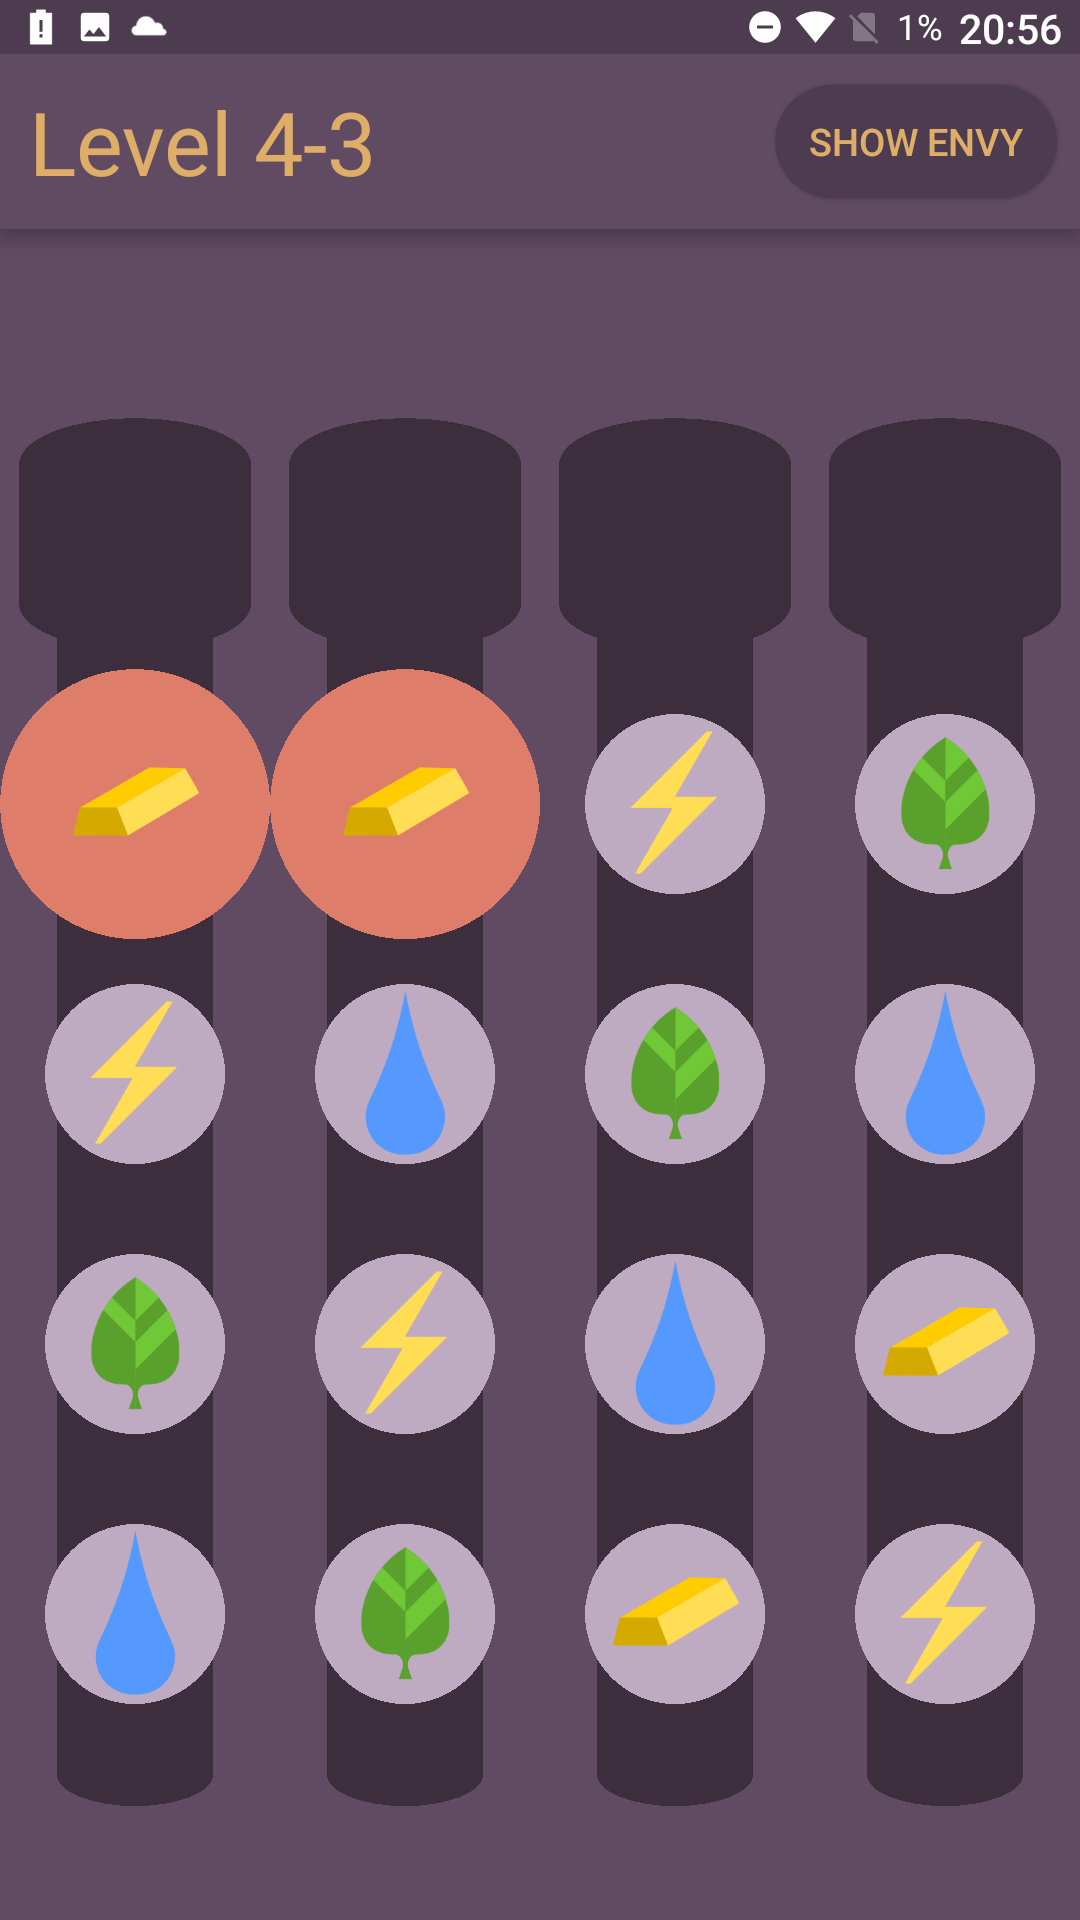
\includegraphics[height=2.5in]{g2}
        \caption{sélection}
    \end{subfigure}%
        \begin{subfigure}[c]{0.23\textwidth}
        \centering
        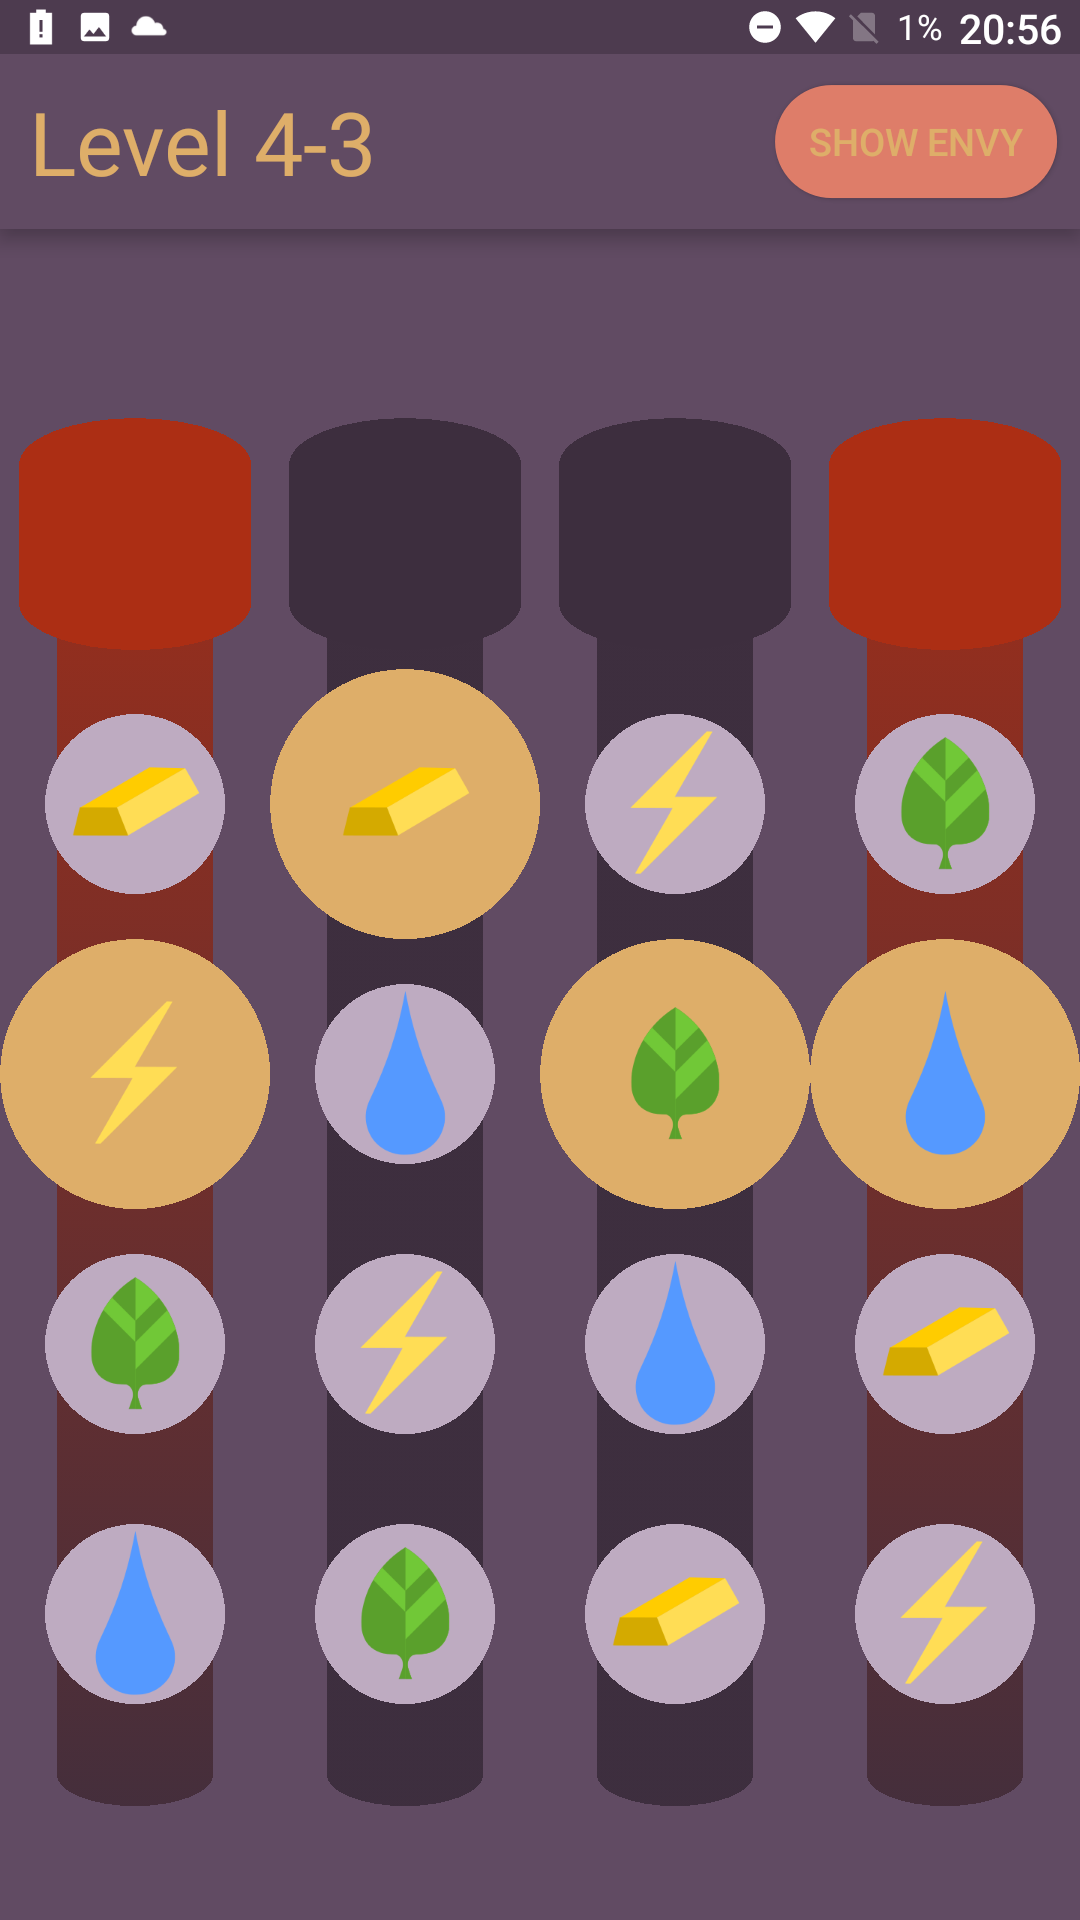
\includegraphics[height=2.5in]{g3}
        \caption{affichag}
    \end{subfigure}%
    \begin{subfigure}[d]{0.23\textwidth}
        \centering
        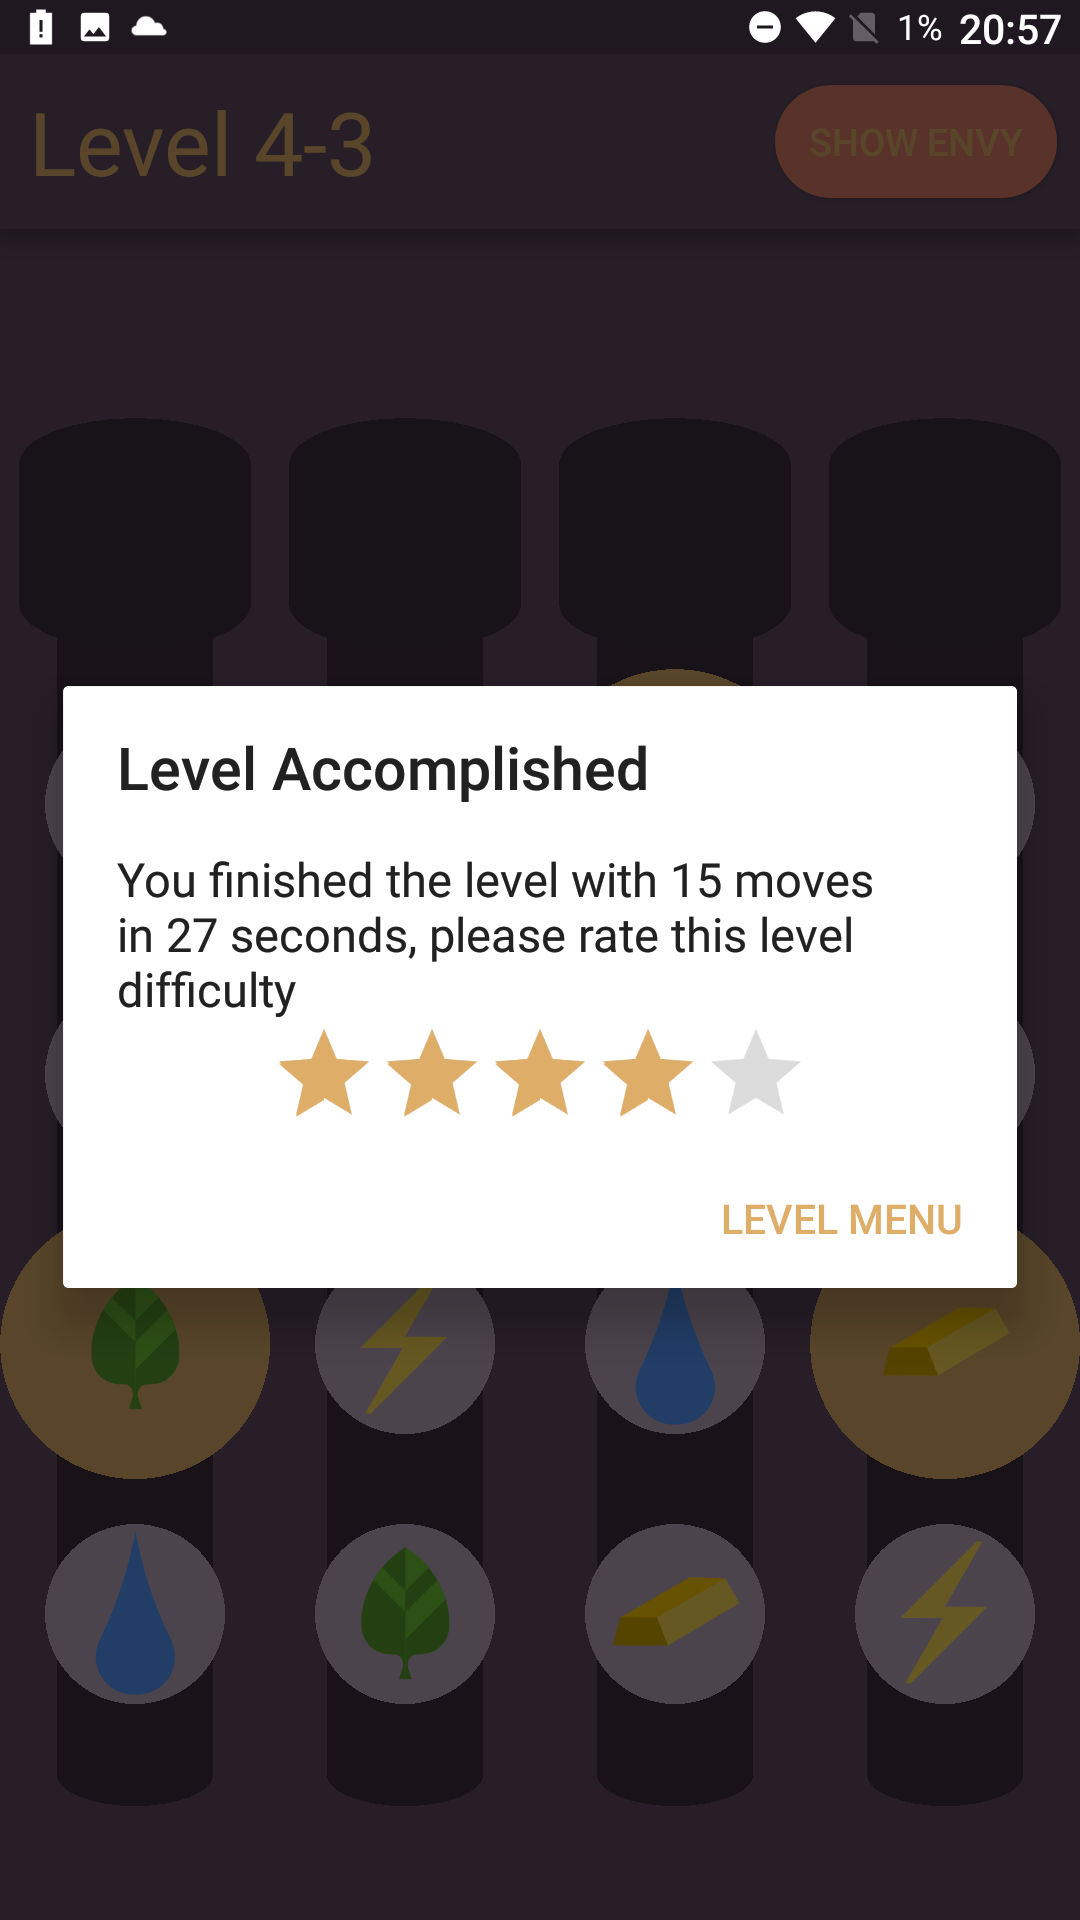
\includegraphics[height=2.5in]{g4}
        \caption{victoire}
    \end{subfigure}
    \caption{Exemple Gameview}
\end{figure}

	\subsection{Récupération des données}
	
	\paragraph{}
	L’analyse de diverses instances du problème nous a permis donc de dégager plusieurs métriques, qui peuvent être utilisées pour essayer de prédire la difficulté de nos niveaux. Cependant, il nous fallait confronter ces prédictions avec des données réelles , qui seraient justement basé sur ces critères, et ce afin de trouver si oui ou non, il existait une corrélation entre la difficulté d’un niveau et ces derniers. 
	\paragraph{}
Une fois l’application mobile réalisée, nous avions donc décidé de la faire tester sur un public de taille variante et diverse, pour recueillir assez de données. Mais nous avions besoin d’un moyen de les écrire quelque part , la contrainte étant que l’utilisateur allait jouer sur son téléphone. Il nous fallait donc envoyer ces informations sur une sorte de base de données. Notre regard s’est alors porté sur l’API Google Sheets qui nous offrait une relaxation de cette contrainte.

\paragraph{Googlesheets}
Nous avons donc intégré dans l’application mobile, une solution permettant l’envois de diverses données joueurs qui étaient enregistrées lors de la résolution d’une instance : l’API Google Sheets permet l’écriture/lecture de données sur une Google Sheet via différentes plateformes : application mobile, site web, programme python, etc….. 
En ce qui nous concerne, notre but est d’envoyer les différentes métriques abordées précédemment sur une Google Sheet avec diverses informations sur l’utilisateur pour ensuite les analyser et appliquer une régression dessus.

\paragraph{}
La communication entre la feuille et notre application est géré via l’API, et elle est sécurisé. En effet l’API utilise le protocole OAuth 2.0 pour autoriser les communications. Nous avons donc besoins d’identifiants , deux moyen sont disponibles :
 \begin{itemize}
\item l’usage d’une Clé API
\item l’usage d’un compte de service Google
\end{itemize}
Néanmoins, la première méthode requiert une confirmation de l’utilisateur à chaque fois qu’il envoie des données via son téléphone car l’application demandera la permission d'interagir avec la feuille sous le compte de l’utilisateur. Nous avons donc opté pour la seconde solution qui user d’un compte de service dédié à notre application. L’application interagira via ce compte sans demander la confirmation de l’utilisateur, ce qui est crucial pour l’envie de l’utilisateur à vouloir tester notre application sur une courte durée/longue durée.
Dans les deux cas, un fichier JSON est créé et il contiendra les informations nécessaire pour créer nos identifiants.

\paragraph{}
L’intégration de cette solution dans notre application se traduit donc par deux classes:
 \begin{itemize}
\item La classe SheetsServiceUtil
\item La classe GoogleSheetsWriteUtil
\end{itemize}
\paragraph{}
La première classe java SheetsServiceUtil contient une unique méthode getSheetsService qui permet la création d’une instance de l’objet Sheet qui est l'intermédiaire pour écrire et lire via l’API. Cette instance contiendra les identifiants nécessaire à l’autorisation de la communication entre l’application et la feuille.
\paragraph{}
La deuxième classe java GoogleSheetsWriteUtil contient toutes les méthodes qui seront appelées pour l’écritures de nos données. 
La méthode setup() permet entre autre la création d’une instance de l’objet Credential, à partir de notre fichier JSON qui est contenu dans les ressources de notre applications (pour rappel, on accède aux ressources de nos applications via ctx.getRessourses();). Cette instance est ensuite passée en paramètre dans la méthode getSheetsService de notre classe SheetsServiceUtil qui retournera un objet Sheets, sur lequel toute nos méthodes agiront par la suite.
Par ailleurs, nous récupérons aussi les données du profil utilisateur enregistré si elles existent pour permettre de détecter la modification d’un profil.
\paragraph{}
Nous utilisons des AsyncTask pour envoyer nos données. En effet il est impossible sous android de faire des opérations réseaux ( transfert de données ) , sous le thread principale, on utilise donc des AsyncTask pour le faire en background. Cela nous évite des lags au niveau de l’interface qui est entièrement gérée par le main thread.
et ça reste invisible à l’oeil de l’utilisateur ce qui est à nouveau crucial quant au côté agréable et fluide de son expérience.
\paragraph{}
Nous avons donc trois static private Class dans SheetsServiceUtil qui héritent tous de la class AsyncTask , une classe d’Android qui permet de lancer des threads aisément : 
 \begin{itemize}
\item WriteUserInfoAsyncTask
\item ModifyUserInfoAsyncTask
\item WriteUserEvalAsyncTask
\end{itemize}
Ces trois classes implémentent ainsi la méthode protected doInBackground , qui prend en paramètre un string data, c’est à dire les données à envoyer, et qui permet leur exécution en tâche de fond.
Nous appelons donc à l'intérieure les méthodes de l’API de Google Sheets pour update (pour modifyUserInfoAsync) 
ou écrire de nouvelles données (pour WriteUserEvalAsyncTask et ModifyUserInfoAsyncTask) dans notre feuille en utilisant l’instance de la classe Sheets que l’on avait créé au préalable.
\hfill \break 
\begin{lstlisting}
    private static class WriteUserInfoAsyncTask extends AsyncTask<String, Void, Void> {
        @Override
        protected Void doInBackground(String... data) {

            ValueRange body = new ValueRange()
                    .setValues(Arrays.<List<Object>>asList(
                            new List[]{Arrays.asList(data)}
                    ));
            try {
            	AppendValuesResponse result = sheetsService.spreadsheets().values()
                        .append(SPREADSHEET_ID, "User_Info_2!A1", body)
                        .setValueInputOption("USER_ENTERED")
                        .execute();
            	Object userPos = result.getUpdates().get("updatedRange");
                prefs.edit().putString("userPos", (String) userPos).apply();
            } catch (IOException e) {
                Log.w("GoogleSheet", "Error during user info write; rescheduling");
                failedUserInfo = data;
                e.printStackTrace();
            }
            return null;
        }
    }
\end{lstlisting}
Fonction WriteUserInfoAsyncTask
\paragraph{}
Comme il est possible que l’écriture des données sur la feuille puisse échouer (problème de réseau, téléphone non connecté à internet, etc...) , il est nécessaire de sauvegarder les données non envoyées pour permettre une planification d’un renvois plus tard. Il existe donc deux variables dans notre classe SheetsServiceUtil pour cela : 
failedEvaluation si l’écriture d’une évaluation échoue
failedUserInfo si l’écriture/modification du profil utilisateur échoue
\paragraph{}
Avant toute nouvelles écritures, il faut donc vérifier s’il n’en existe pas qui ont échouées.
Pour cette raison, nous avons créé trois méthodes : WriteUserInfo(String data), ModifyUserInfo(String data) , WriterUserEval(String data), qui appelle toujours au début une méthode “CheckFailures” qui verifie si failedEvaluation et failedUserInfo sont vide ou non. Si elles ne le sont pas, alors on crée de nouvelles asyncTask pour renvoyer ces données. Et dans tous les cas, on crée de nouvelles AsyncTask correspondant à la méthode qui est appelé (par exemple WriteUserInfoAsyncTask pour la méthode WriteUserInfo) pour les nouvelles données passées en paramètre de ces méthodes.
\hfill \break
\begin{lstlisting}
	public void writeUserEvaluation(String... data) {
        	this.checkFailures();
        	new WriteUserEvaluationAsyncTask().execute(data);
    	}
\end{lstlisting}
Méthode WriteUserEvaluation
	
\end{document}



